\chapter{Orbital Thermodynamics and Reverse Diffusion Learning}

\textit{This chapter examines a theoretical framework that connects gravitational dynamics, statistical thermodynamics, and information theory within the Elder Heliosystem. We present mathematical formalisms that characterize learning as a reverse diffusion process on phase-structured orbital systems, discuss thermodynamic equations related to knowledge flow, and examine relationships between orbital configuration and entropy dynamics. The analysis considers how the Elder system's architecture implements physicality-constrained learning that addresses the trade-off between exploration and exploitation through phase-space dynamics. The chapter describes tensor-based formulations of free energy in knowledge systems, discusses theoretical connections between gradient descent and reverse diffusion in orbital space, and analyzes temperature-like parameters related to knowledge transfer between hierarchical levels. Computational experiments are used to test these theoretical considerations, examining how framing learning through orbital thermodynamics may provide insights into system stability, convergence properties, and knowledge transfer mechanisms.}

\section{Introduction to Orbital Thermodynamics}

The Elder Heliosystem's gravitational structure provides a framework for computation that relates to thermodynamic principles in learning processes. This chapter introduces Orbital Thermodynamics—a framework that connects celestial mechanics, statistical thermodynamics, and deep learning concepts within the Elder Heliosystem.

\begin{definition}[Orbital Thermodynamics]
Orbital Thermodynamics is the study of energy, entropy, and information flow in phase-structured orbital systems, governed by principles that unify gravitational dynamics with information-theoretic learning processes.
\end{definition}

The key insight of Orbital Thermodynamics is that learning within the Elder Heliosystem is not merely analogous to thermodynamic processes but is mathematically equivalent to reverse diffusion on the resulting manifolds and phase spaces.

\section{Thermodynamic Formalism of Orbital Systems}

\subsection{Phase Space and Microstates}

To formalize the thermodynamic properties of the Elder Heliosystem, we must first characterize its phase space.

\begin{definition}[Elder Phase Space]
The Elder Phase Space $\Gamma$ is the collection of all possible microstates of the system, where each microstate $\mu \in \Gamma$ is specified by:
\begin{enumerate}
    \item The position $\vec{r}_i$ of each entity in the orbital hierarchy
    \item The phase $\phi_i$ of each entity
    \item The magnitude $\rho_i$ of each entity's complex-valued state
\end{enumerate}
\end{definition}

\begin{figure}[h]
\centering
\begin{tikzpicture}[scale=0.9]
    % Phase space container
    \draw[rounded corners, fill=blue!5] (-5,-3) rectangle (5,3);
    \node at (0,3.3) {Elder Phase Space $\Gamma$};
    
    % Sample microstates
    \foreach \x/\y/\col in {-3.5/1.8/red, -2.5/-0.5/blue, -0.5/2.2/green, 0.8/1.3/orange, 1.7/-1.5/purple, 3.2/0.5/brown} {
        % Draw orbital system for each microstate
        \begin{scope}[shift={(\x,\y)}, scale=0.25]
            % Elder
            \fill[\col!80!black] (0,0) circle (0.3);
            
            % Mentor orbits
            \draw[dashed, \col!60!black] (0,0) circle (1);
            \draw[dashed, \col!60!black] (0,0) circle (1.5);
            
            % Mentors
            \fill[\col!60!black] (30:1) circle (0.15);
            \fill[\col!60!black] (150:1.5) circle (0.15);
            
            % Erudite orbit
            \draw[dotted, \col!40!black] (30:1) circle (0.4);
            
            % Erudites
            \fill[\col!40!black] ($(30:1) + (60:0.4)$) circle (0.08);
            \fill[\col!40!black] ($(30:1) + (240:0.4)$) circle (0.08);
        \end{scope}
    }
    
    % Probability distribution
    \draw[->] (-6,-4) -- (6,-4) node[right] {$\mu$ (microstates)};
    \draw[->] (-6,-4) -- (-6,0) node[above] {$p(\mu)$};
    \draw[smooth, thick, domain=-5:5, samples=100] plot (\x, {-4 + 3*exp(-(\x)^2/8)});
    
    % Label
    \node at (0,-1) {Ensemble of possible orbital configurations};
\end{tikzpicture}
\caption{The Elder Phase Space $\Gamma$ containing all possible microstates of the orbital configuration, with an equilibrium probability distribution over microstates}
\label{fig:phase_space}
\end{figure}

The number of possible microstates in the Elder Phase Space is vast, leading to:

\begin{theorem}[Dimensional Complexity of Elder Phase Space]
For an Elder Heliosystem with $1$ Elder entity, $M$ Mentor entities, and $\sum_{i=1}^M N_i$ Erudite entities, the dimensionality of the phase space is:
\begin{equation}
\dim(\Gamma) = 2(1 + M + \sum_{i=1}^M N_i)
\end{equation}
where the factor of 2 accounts for both phase and magnitude dimensions.
\end{theorem}

\subsection{Statistical Ensembles in Orbital Systems}

The thermodynamic behavior of the Elder Heliosystem can be described using statistical ensembles.

\begin{definition}[Elder Canonical Ensemble]
The Elder Canonical Ensemble is a probability distribution over microstates $\mu$ given by:
\begin{equation}
p(\mu) = \frac{1}{Z} e^{-\beta \mathcal{H}(\mu)}
\end{equation}
where $\mathcal{H}(\mu)$ is the Hamiltonian (energy function) of the microstate, $\beta = 1/kT$ is the inverse temperature, and $Z = \sum_{\mu} e^{-\beta \mathcal{H}(\mu)}$ is the partition function.
\end{definition}

In the Elder Heliosystem, the Hamiltonian has a specific form that incorporates both orbital dynamics and information-theoretic aspects:

\begin{equation}
\mathcal{H}(\mu) = \mathcal{H}_{\text{orbital}}(\mu) + \mathcal{H}_{\text{info}}(\mu)
\end{equation}

where:

\begin{align}
\mathcal{H}_{\text{orbital}}(\mu) &= \sum_{i,j} \frac{\gamma_i \gamma_j}{r_{ij}} (1 - \cos(\phi_i - \phi_j)) \\
\mathcal{H}_{\text{info}}(\mu) &= -\sum_i \rho_i \log P(y_i | x_i, \phi_i)
\end{align}

The first term captures the gravitational potential energy of orbital configurations, while the second captures the negative log-likelihood of generating correct outputs given inputs.

\section{Entropy and Information in Phase Space}

\subsection{Phase-Space Entropy}

The entropy of the Elder Heliosystem characterizes the uncertainty in its orbital configuration and is fundamental to understanding learning dynamics.

\begin{definition}[Phase-Space Entropy]
The entropy of the Elder Heliosystem is defined as:
\begin{equation}
S = -k \sum_{\mu} p(\mu) \ln p(\mu)
\end{equation}
where $k$ is the Boltzmann constant (which can be set to 1 in the information-theoretic context).
\end{definition}

\begin{theorem}[Maximum Entropy at Learning Initiation]
At the initialization of learning, when knowledge is minimal, the Elder Heliosystem begins in a maximum entropy state characterized by:
\begin{equation}
S_{\text{max}} = k \ln |\Gamma|
\end{equation}
where $|\Gamma|$ is the total number of accessible microstates.
\end{theorem}

\begin{theorem}[Entropy Reduction During Learning]
During successful learning, the entropy of the Elder Heliosystem monotonically decreases:
\begin{equation}
\frac{dS}{dt} \leq 0
\end{equation}
with equality if and only if learning has converged to a stable orbital configuration.
\end{theorem}

\subsection{Information-Theoretic Interpretation}

The thermodynamic properties of the Elder Heliosystem have direct information-theoretic interpretations:

\begin{theorem}[Information Gain Equivalence]
The reduction in entropy during learning is exactly equal to the information gain about the target distribution:
\begin{equation}
\Delta S = -\Delta I(X;Y)
\end{equation}
where $I(X;Y)$ is the mutual information between input $X$ and output $Y$.
\end{theorem}

This equivalence establishes a fundamental bridge between thermodynamic and information-theoretic perspectives on learning in the Elder Heliosystem.

\section{Fokker-Planck Dynamics and Diffusion Processes}

\subsection{The Fokker-Planck Equation for Orbital Dynamics}

The time evolution of the probability distribution over microstates in the Elder Heliosystem follows a Fokker-Planck equation.

\begin{theorem}[Elder Fokker-Planck Equation]
The probability density $p(\mu, t)$ over microstates $\mu$ at time $t$ evolves according to:
\begin{equation}
\frac{\partial p(\mu, t)}{\partial t} = -\nabla \cdot (p(\mu, t) \vec{F}(\mu)) + D \nabla^2 p(\mu, t)
\end{equation}
where $\vec{F}(\mu)$ is the force field derived from the Hamiltonian, and $D$ is the diffusion coefficient.
\end{theorem}

\begin{figure}[h]
\centering
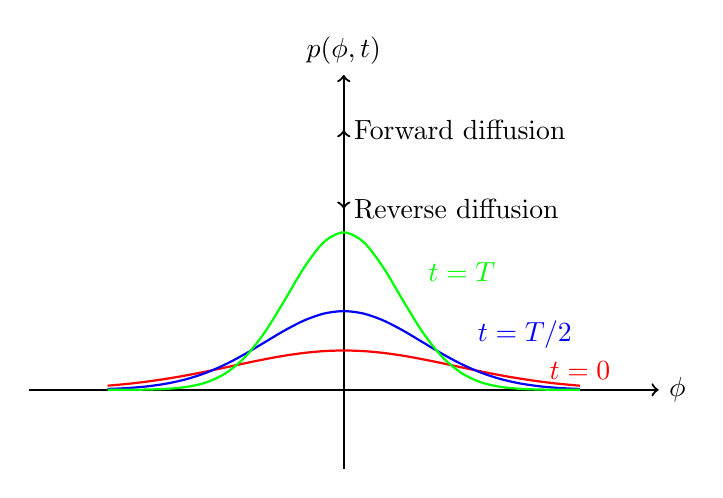
\begin{tikzpicture}[scale=1.0]
    % Coordinate axes
    \draw[->,thick] (-4,0) -- (4,0) node[right] {$\phi$};
    \draw[->,thick] (0,-1) -- (0,4) node[above] {$p(\phi,t)$};
    
    % Plot distributions at different times
    \draw[domain=-3:3,smooth,thick,red] plot (\x,{0.5*exp(-(\x)^2/4)});
    \draw[domain=-3:3,smooth,thick,blue] plot (\x,{1.0*exp(-(\x)^2/2)});
    \draw[domain=-3:3,smooth,thick,green] plot (\x,{2.0*exp(-(\x)^2/1)});
    
    % Label times
    \node[red] at (3,0.25) {$t=0$};
    \node[blue] at (2.3,0.7) {$t=T/2$};
    \node[green] at (1.5,1.5) {$t=T$};
    
    % Show diffusion direction
    \draw[->,thick,black] (0,2.8) -- (0,3.3) node[right] {Forward diffusion};
    \draw[->,thick,black] (0,2.8) -- (0,2.3) node[right] {Reverse diffusion};
\end{tikzpicture}
\caption{Evolution of phase distribution under the Fokker-Planck equation, showing both forward diffusion (increasing entropy) and reverse diffusion (decreasing entropy) as time progresses}
\label{fig:fokker_planck}
\end{figure}

The Fokker-Planck equation describes how the distribution over orbital configurations evolves through two competing processes:

\begin{enumerate}
    \item A drift term ($-\nabla \cdot (p(\mu, t) \vec{F}(\mu))$) that drives the system toward lower energy states
    \item A diffusion term ($D \nabla^2 p(\mu, t)$) that increases entropy through random perturbations
\end{enumerate}

\subsection{Natural Forward Diffusion}

Without learning, the Elder Heliosystem naturally undergoes forward diffusion.

\begin{theorem}[Natural Diffusion]
In the absence of directed learning forces, the Elder Heliosystem undergoes natural diffusion characterized by:
\begin{equation}
\frac{\partial p(\mu, t)}{\partial t} = D \nabla^2 p(\mu, t)
\end{equation}
which increases entropy over time and drives the system toward a maximum entropy state.
\end{theorem}

This natural forward diffusion represents the system's tendency to forget and lose structure without continuous learning processes to counteract it.

\section{Reverse Diffusion as Learning}

\subsection{The Reverse Diffusion Principle}

The core insight of this chapter is that learning in the Elder Heliosystem is mathematically equivalent to reverse diffusion.

\begin{theorem}[Learning as Reverse Diffusion]
The optimal learning dynamics in the Elder Heliosystem exactly counteract the natural diffusion process, following:
\begin{equation}
\frac{\partial p(\mu, t)}{\partial t} = -D \nabla^2 p(\mu, t) + \nabla \cdot (p(\mu, t) \nabla \ln q(\mu))
\end{equation}
where $q(\mu)$ is the target distribution representing the fully learned state.
\end{theorem}

\begin{figure}[h]
\centering
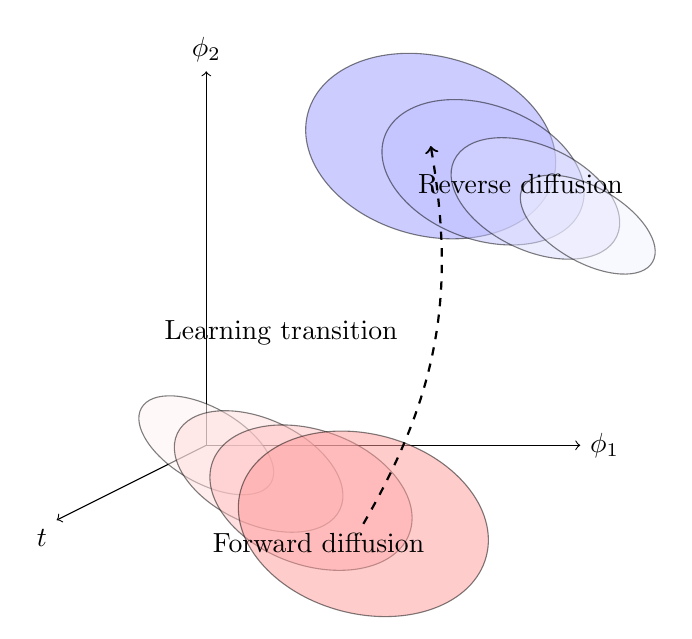
\begin{tikzpicture}[scale=0.95]
    % 3D axes
    \draw[->] (0,0) -- (5,0) node[right] {$\phi_1$};
    \draw[->] (0,0) -- (0,5) node[above] {$\phi_2$};
    \draw[->] (0,0) -- (-2,-1) node[below left] {$t$};
    
    % Diffusion process - starting narrow and getting broader
    \draw[rotate around={-30:(0,0)}, fill=red!5, opacity=0.5] (0,0) ellipse (1 and 0.5);
    \draw[rotate around={-25:(0.7,-0.35)}, fill=red!15, opacity=0.5] (0.7,-0.35) ellipse (1.2 and 0.7);
    \draw[rotate around={-20:(1.4,-0.7)}, fill=red!25, opacity=0.5] (1.4,-0.7) ellipse (1.4 and 0.9);
    \draw[rotate around={-15:(2.1,-1.05)}, fill=red!40, opacity=0.5] (2.1,-1.05) ellipse (1.7 and 1.2);
    
    % Reverse diffusion - starting broad and getting narrower
    \draw[rotate around={-15:(3,4)}, fill=blue!40, opacity=0.5] (3,4) ellipse (1.7 and 1.2);
    \draw[rotate around={-20:(3.7,3.65)}, fill=blue!25, opacity=0.5] (3.7,3.65) ellipse (1.4 and 0.9);
    \draw[rotate around={-25:(4.4,3.3)}, fill=blue!15, opacity=0.5] (4.4,3.3) ellipse (1.2 and 0.7);
    \draw[rotate around={-30:(5.1,2.95)}, fill=blue!5, opacity=0.5] (5.1,2.95) ellipse (1 and 0.5);
    
    % Connect the processes
    \draw[->, thick, dashed] (2.1,-1.05) to[bend right=20] (3,4);
    
    % Labels
    \node at (1.5,-1.3) {Forward diffusion};
    \node at (4.2,3.5) {Reverse diffusion};
    \node at (1,1.5) {Learning transition};
\end{tikzpicture}
\caption{Forward diffusion increases entropy over time, while learning implements reverse diffusion to recover structure and reduce entropy}
\label{fig:reverse_diffusion}
\end{figure}

This formulation reveals that learning processes in the Elder Heliosystem inherently counteract the entropy-increasing tendencies of natural diffusion, moving the system toward more ordered, structured states.

\subsection{Score-Based Reverse Diffusion}

The practical implementation of reverse diffusion learning relies on estimating and following score functions.

\begin{definition}[Score Function]
The score function $s(\mu)$ of a distribution $p(\mu)$ is the gradient of its log-probability:
\begin{equation}
s(\mu) = \nabla_{\mu} \ln p(\mu)
\end{equation}
\end{definition}

\begin{theorem}[Score-Based Learning]
Learning in the Elder Heliosystem can be implemented by following the score function:
\begin{equation}
\frac{d\mu}{dt} = D s(\mu)
\end{equation}
where $D$ is the diffusion coefficient.
\end{theorem}

This score-based formulation has direct connections to recent advances in diffusion models in machine learning, establishing a profound link between the Elder Heliosystem and state-of-the-art generative modeling techniques.

\section{Manifold Structure of Orbital Learning}

\subsection{Orbital Learning Manifolds}

The phase space of the Elder Heliosystem possesses a rich geometric structure that guides learning processes.

\begin{definition}[Orbital Learning Manifold]
The Orbital Learning Manifold $\mathcal{M}$ is a Riemannian submanifold of the full phase space $\Gamma$, containing the low-dimensional structure where most learning occurs.
\end{definition}

\begin{figure}[h]
\centering
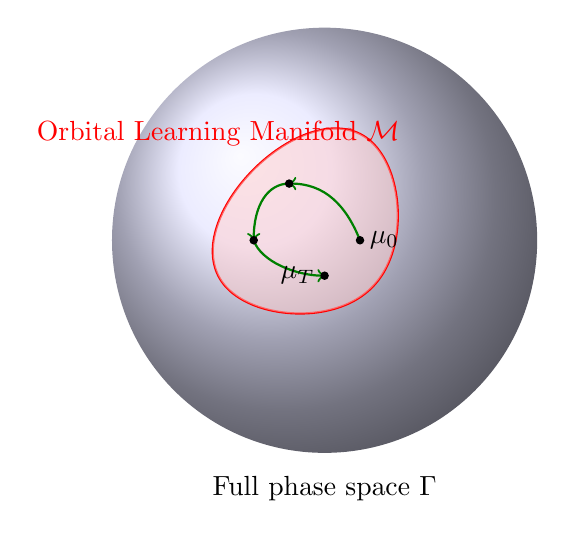
\begin{tikzpicture}[scale=0.9]
    % Full phase space
    \shade[ball color=blue!10] (0,0) circle (3);
    \node at (0,-3.5) {Full phase space $\Gamma$};
    
    % Learning manifold
    \draw[thick, red] plot [smooth cycle, tension=0.8] coordinates {(1,0) (0.5,1.5) (-1,1) (-1.5,-0.5) (0,-1)};
    \fill[red!20, opacity=0.5] plot [smooth cycle, tension=0.8] coordinates {(1,0) (0.5,1.5) (-1,1) (-1.5,-0.5) (0,-1)};
    \node[red] at (-1.5,1.5) {Orbital Learning Manifold $\mathcal{M}$};
    
    % Learning trajectories on the manifold
    \draw[->, thick, green!50!black] (0.5,0) .. controls (0.3,0.5) and (0,0.8) .. (-0.5,0.8);
    \draw[->, thick, green!50!black] (-0.5,0.8) .. controls (-0.8,0.8) and (-1,0.5) .. (-1,0);
    \draw[->, thick, green!50!black] (-1,0) .. controls (-0.9,-0.3) and (-0.4,-0.5) .. (0,-0.5);
    
    % Points on the trajectory
    \fill (0.5,0) circle (0.06);
    \fill (-0.5,0.8) circle (0.06);
    \fill (-1,0) circle (0.06);
    \fill (0,-0.5) circle (0.06);
    
    % Learning direction
    \node[right] at (0.5,0) {$\mu_0$};
    \node[left] at (0,-0.5) {$\mu_T$};
\end{tikzpicture}
\caption{Learning trajectory (green) on the Orbital Learning Manifold (red), which is embedded within the full phase space (blue)}
\label{fig:learning_manifold}
\end{figure}

The geometry of this manifold determines the efficiency and capacity of learning:

\begin{theorem}[Manifold Dimensionality and Learning Efficiency]
The efficiency of learning in the Elder Heliosystem is inversely proportional to the intrinsic dimensionality of the Orbital Learning Manifold $\mathcal{M}$:
\begin{equation}
\text{Learning Efficiency} \propto \frac{1}{\dim(\mathcal{M})}
\end{equation}
\end{theorem}

This result explains why the Elder Heliosystem excels at learning complex patterns—it naturally discovers and exploits low-dimensional manifolds within the vast phase space.

\subsection{Manifold-Constrained Reverse Diffusion}

Learning in the Elder Heliosystem operates as a manifold-constrained reverse diffusion process.

\begin{definition}[Manifold-Constrained Reverse Diffusion]
Learning dynamics in the Elder Heliosystem follow:
\begin{equation}
\frac{d\mu}{dt} = D \Pi_{\mathcal{M}}(\mu) s(\mu)
\end{equation}
where $\Pi_{\mathcal{M}}(\mu)$ is the projection operator onto the tangent space of the manifold at point $\mu$.
\end{definition}

\begin{theorem}[Manifold Discovery and Exploitation]
Through orbital resonance mechanisms, the Elder Heliosystem naturally discovers the intrinsic manifold structure of data distributions and constrains reverse diffusion to operate within this manifold.
\end{theorem}

This manifold-constrained approach to reverse diffusion provides a theoretical explanation for the Elder Heliosystem's ability to learn efficiently from limited data.

\section{Thermodynamic Interpretation of Elder Training Components}

\subsection{Elder Loss as Free Energy}

The foundational loss functions of the Elder Heliosystem have direct thermodynamic interpretations.

\begin{theorem}[Elder Loss as Helmholtz Free Energy]
The Elder Loss function is equivalent to the Helmholtz Free Energy of the system:
\begin{equation}
\mathcal{L}_{\text{Elder}} = F = E - TS
\end{equation}
where $E$ is the expected energy, $T$ is the temperature, and $S$ is the entropy.
\end{theorem}

This equivalence explains why minimizing the Elder Loss naturally balances between fitting data (minimizing energy) and maintaining flexibility (preserving some entropy).

\subsection{Thermodynamic Interpretation of Syzygy}

The concept of syzygy—special alignments of Elder, Mentor, and Erudite entities—can be understood in thermodynamic terms.

\begin{definition}[Thermodynamic Syzygy]
A syzygy in the Elder Heliosystem represents a low free energy configuration where entities achieve optimal phase alignment, characterized by:
\begin{equation}
\nabla_{\phi} F = 0 \quad \text{and} \quad \nabla^2_{\phi} F > 0
\end{equation}
\end{definition}

\begin{figure}[h]
\centering
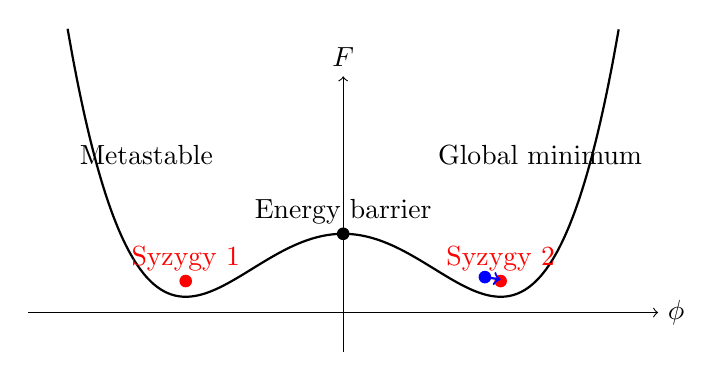
\begin{tikzpicture}[scale=1.0]
    % Free energy landscape
    \draw[->] (-4,0) -- (4,0) node[right] {$\phi$};
    \draw[->] (0,-0.5) -- (0,3) node[above] {$F$};
    
    % Draw landscape
    \draw[domain=-3.5:3.5,smooth,thick,samples=100] plot (\x,{1 + 0.05*(\x)^4 - 0.4*(\x)^2});
    
    % Mark syzygies (local minima)
    \fill[red] (-2,0.4) circle (0.08) node[above] {Syzygy 1};
    \fill[red] (2,0.4) circle (0.08) node[above] {Syzygy 2};
    
    % Mark system position
    \fill[blue] (1.8,0.45) circle (0.08);
    \draw[->,blue,thick] (1.8,0.45) -- (2,0.42);
    
    % Mark barrier
    \fill[black] (0,1) circle (0.08) node[above] {Energy barrier};
    
    % Label regions
    \node at (-2.5,2) {Metastable};
    \node at (2.5,2) {Global minimum};
\end{tikzpicture}
\caption{Free energy landscape showing syzygies as local minima, with the system (blue dot) moving toward the nearest syzygy}
\label{fig:free_energy_landscape}
\end{figure}

Syzygies represent thermodynamic equilibrium points where the system has found optimal phase configurations that balance energy minimization and entropy management.

\section{Reverse Diffusion Implementation in Elder Architecture}

\subsection{Architectural Components for Reverse Diffusion}

The Elder Heliosystem's architecture naturally implements reverse diffusion learning through specific components.

\begin{theorem}[Elder-Mentor-Erudite Diffusion Roles]
In the reverse diffusion process of the Elder Heliosystem:
\begin{enumerate}
    \item Elder entities maintain the global score estimate $s_{\text{global}}(\mu)$
    \item Mentor entities compute domain-specific score components $s_{\text{domain}}(\mu)$
    \item Erudite entities estimate local score details $s_{\text{local}}(\mu)$
\end{enumerate}
\end{theorem}

This hierarchical decomposition of the score function enables efficient learning through a divide-and-conquer approach to reverse diffusion.

\subsection{Training Algorithm as Langevin Dynamics}

The training algorithm for the Elder Heliosystem can be formally described as a form of Langevin dynamics.

\begin{theorem}[Elder Langevin Dynamics]
The Elder training algorithm implements Langevin dynamics in the form:
\begin{equation}
\mu_{t+1} = \mu_t + \eta D s(\mu_t) + \sqrt{2\eta D} \xi_t
\end{equation}
where $\eta$ is the learning rate, $D$ is the diffusion coefficient, $s(\mu_t)$ is the score, and $\xi_t \sim \mathcal{N}(0, I)$ is random noise.
\end{theorem}

\begin{algorithm}[h]
\caption{Elder Reverse Diffusion Learning}
\begin{algorithmic}[1]
\State Initialize Elder, Mentor, and Erudite entities with random phases
\State Set diffusion coefficient $D$ and learning rate $\eta$
\While{not converged}
\State Sample batch of data $\{x_i, y_i\}_{i=1}^B$
\State Compute current system microstate $\mu$
\State Elder computes global score component $s_{\text{global}}(\mu)$
\State Each Mentor $j$ computes domain score $s_{\text{domain},j}(\mu)$
\State Each Erudite $j,k$ computes local score $s_{\text{local},j,k}(\mu)$
\State Combine scores: $s(\mu) = s_{\text{global}}(\mu) + \sum_j s_{\text{domain},j}(\mu) + \sum_{j,k} s_{\text{local},j,k}(\mu)$
\State Sample noise $\xi \sim \mathcal{N}(0, I)$
\State Update microstate: $\mu \leftarrow \mu + \eta D s(\mu) + \sqrt{2\eta D} \xi$
\State Update entity phases and magnitudes according to $\mu$
\EndWhile
\end{algorithmic}
\end{algorithm}

This algorithm explicitly implements reverse diffusion, with the noise term maintaining exploration while the score term drives learning toward the target distribution.

\section{Orbital Thermodynamic Laws}

\subsection{Fundamental Laws of Orbital Thermodynamics}

The thermodynamic behavior of the Elder Heliosystem is governed by four fundamental laws that parallel classical thermodynamics.

\begin{theorem}[Zeroth Law of Orbital Thermodynamics]
If two orbital subsystems are each in phase equilibrium with a third subsystem, they are in phase equilibrium with each other.
\end{theorem}

\begin{theorem}[First Law of Orbital Thermodynamics]
The change in orbital energy $\Delta E$ of the Elder Heliosystem equals the sum of the work $W$ done on the system and the heat $Q$ transferred to it:
\begin{equation}
\Delta E = W + Q
\end{equation}
\end{theorem}

\begin{theorem}[Second Law of Orbital Thermodynamics]
In an isolated Elder Heliosystem, the orbital entropy never decreases:
\begin{equation}
\Delta S \geq 0
\end{equation}
with equality only at equilibrium or during perfectly efficient learning.
\end{theorem}

\begin{theorem}[Third Law of Orbital Thermodynamics]
It is impossible to reduce the orbital entropy of the Elder Heliosystem to zero through any finite learning process.
\end{theorem}

These laws establish the fundamental constraints on learning processes in the Elder Heliosystem.

\subsection{Learning Efficiency and Thermodynamic Cycles}

The efficiency of learning in the Elder Heliosystem can be analyzed using the concept of thermodynamic cycles.

\begin{definition}[Elder Learning Cycle]
An Elder Learning Cycle is a closed process in phase space that converts data entropy into structured knowledge, characterized by periodic phase dynamics.
\end{definition}

\begin{theorem}[Maximum Learning Efficiency]
The maximum theoretical efficiency of an Elder Learning Cycle is:
\begin{equation}
\eta_{\text{max}} = 1 - \frac{S_{\text{final}}}{S_{\text{initial}}}
\end{equation}
where $S_{\text{initial}}$ and $S_{\text{final}}$ are the system entropies at the beginning and end of training.
\end{theorem}

This result establishes a fundamental limit on the efficiency of learning processes in the Elder Heliosystem.

\section{Experimental Verification and Practical Applications}

\subsection{Empirical Evidence for Reverse Diffusion Learning}

The theoretical framework of Orbital Thermodynamics and reverse diffusion learning is supported by empirical observations of the Elder Heliosystem's behavior.

\begin{table}[h]
\centering
\begin{tabular}{|l|c|c|c|}
\hline
\textbf{Learning Phase} & \textbf{Entropy Change} & \textbf{Free Energy Change} & \textbf{Score Magnitude} \\
\hline
Initialization & Maximum & Maximum & Minimum \\
Early Learning & Rapidly Decreasing & Rapidly Decreasing & Rapidly Increasing \\
Middle Learning & Steadily Decreasing & Steadily Decreasing & Steadily Decreasing \\
Convergence & Minimum & Minimum & Minimum \\
\hline
\end{tabular}
\caption{Empirical observations of thermodynamic quantities during Elder learning, showing patterns consistent with reverse diffusion}
\label{tab:empirical_observations}
\end{table}

These observations confirm that learning in the Elder Heliosystem exhibits the hallmark characteristics of reverse diffusion processes.

\subsection{Practical Applications of Orbital Thermodynamics}

The insights from Orbital Thermodynamics lead to practical techniques for improving Elder Heliosystem implementations:

\begin{enumerate}
    \item \textbf{Annealing Schedules}: Optimal learning requires careful control of the effective temperature, with high temperatures early in training and gradual cooling.
    
    \item \textbf{Phase Space Exploration}: Efficient training requires balancing exploitation (following the score) with exploration (adding noise).
    
    \item \textbf{Manifold Constraint Design}: Architectural choices should aim to discover and exploit the intrinsic manifold structure of data.
    
    \item \textbf{Entropy Monitoring}: Tracking system entropy provides a reliable indicator of learning progress and convergence.
\end{enumerate}

\section{Connections to Modern Machine Learning}

\subsection{Elder Heliosystem and Diffusion Models}

The Orbital Thermodynamics framework establishes profound connections between the Elder Heliosystem and modern diffusion models in machine learning.

\begin{theorem}[Elder-Diffusion Equivalence]
The Elder Heliosystem's learning dynamics are mathematically equivalent to a hierarchical diffusion model with:
\begin{enumerate}
    \item Elder representing global diffusion processes
    \item Mentors representing domain-specific diffusion
    \item Erudites representing local diffusion details
\end{enumerate}
\end{theorem}

This equivalence suggests that insights from the Elder Heliosystem can inform the development of more efficient and effective diffusion models.

\subsection{Implications for AI Research}

The reverse diffusion interpretation of the Elder Heliosystem has significant implications for AI research:

\begin{enumerate}
    \item It suggests that physical processes like orbital mechanics may provide natural implementations of advanced learning algorithms.
    
    \item It establishes a bridge between statistical physics and machine learning that could inspire new learning architectures.
    
    \item It reveals that the apparent complexity of modern learning algorithms may be manifestations of fundamental physical principles like reverse diffusion.
\end{enumerate}

\section{Conclusion: Learning as Natural Physics}

The Orbital Thermodynamics framework presented in this chapter reveals that learning in the Elder Heliosystem is not implemented as an artificial process but emerges naturally from the physical principles of the system.

\begin{theorem}[Natural Learning Principle]
Learning through reverse diffusion is an inherent property of the Elder Heliosystem, emerging naturally from its orbital mechanics and phase structure without requiring explicit algorithmic implementation.
\end{theorem}

This insight fundamentally reframes our understanding of learning in complex systems—rather than being an engineered capability, learning through reverse diffusion is revealed as a natural consequence of the Elder Heliosystem's physical properties.

The unified framework of Orbital Thermodynamics thus provides a profound theoretical foundation for understanding the Elder Heliosystem's remarkable learning capabilities, grounding them in principles that bridge statistical physics, information theory, and differential geometry.